% 
% (c) Copyright 2016 Tabea Mendez
% 
% This source is free: you can redistribute it and/or modify
% it under the terms of the GNU General Public License as published by
% the Free Software Foundation, either version 3 of the License, or
% (at your option) any later version.
% 
% This source is distributed in the hope that it will be useful,
% but WITHOUT ANY WARRANTY; without even the implied warranty of
% MERCHANTABILITY or FITNESS FOR A PARTICULAR PURPOSE.  See the
% GNU General Public License for more details.
% 
% You should have received a copy of the GNU General Public License
% along with this source.  If not, see <http://www.gnu.org/licenses/>.
%
%%%%%%%%%%%%%%%%%%%%%%%%%%%%%%%%%%%%%%%%%%%%%%%%%%%%%%%%%%%%%%%%%%%%%%%%%%%%%%

\section{Blockverarbeitungsmethoden}
	\begin{minipage}{0.65\textwidth}
		Oft werden analoge Signale eine bestimmte Zeit lang abgetastet und in einem Vektor gespeichert. Dieser wird dann als Block verarbeitet.\\[0.2cm]
		\textbf{Messdauer:}$\qquad\qquad\;\;$\fcolorbox{CadetRed}{white}{$T_{Lx} = L_x\cdot T$}\\[0.2cm]
		\textbf{Anzahl Samples:}$\qquad$\fcolorbox{CadetRed}{white}{$L_x = T_{Lx}\cdot f_s$}
	\end{minipage}\begin{minipage}{0.05\textwidth}$ $\end{minipage}
	\begin{minipage}{0.3\textwidth}
		\begin{tikzpicture}[>=latex', scale=1.4]
			\def\s{0.4};
			\def\l{1};
			\def\d{0};

			\coordinate (f2) at (0,0);
			\draw[line width=0.5,->](f2)++(-1.5,0)--++(3.1,0)node[right]{\footnotesize$n$};
			\draw[line width=0.5,->](f2)++({(-3-1)/4+\d},-0.1)node[below]{\footnotesize$0$}--++(0,\l+0.1)node[right]{\footnotesize $x(n)$};
			\foreach \i in {-3,...,4}
			{
				\draw[line width=1,fill](f2)++({(\i-1)/4+\d},0)--++(0,{0.3*cos(\i*0.55*180/pi)+0.4})circle(0.04);
			}
			\draw[line width=1,fill](f2)++({(5-1)/4+\d},0)node[below]{\footnotesize$L_x$-$1$}--++(0,{0.3*cos(5*0.55*180/pi)+0.4})circle(0.04);

			\draw[line width=0.5,fill](f2)++({(6-1)/4+\d},0.1)--++(0,{-0.2});

			\draw[line width=0.5, black](f2)++({-(5-1)/4+\d},-0.4)--++(0,-0.2);
			\draw[line width=0.5, black,<->](f2)++({-(5-1)/4+\d},-0.5)--node[above]{\footnotesize$T_{Lx}$}++({2*(5.5-1)/4+\d},0);
			\draw[line width=0.5, black](f2)++({-(5-1)/4+\d},-0.5)++({2*(5.5-1)/4+\d},0)--++(0,0.1)--++(0,-0.2)--++(0,0.1);

			\coordinate (f2) at (0,0.8);
			\draw[line width=0.5](f2)++({(3-1)/4+\d},0.1)--node[fill=white]{\footnotesize$T$}++(-0.25,0);
			\draw[line width=0.5, black](f2)++({(2-1)/4+\d},0)--++(0,0.2);
			\draw[line width=0.5, black](f2)++({(3-1)/4+\d},0)--++(0,0.2);
			\draw[line width=0.5, black,<-](f2)++({(2-1)/4+\d},0.1)--++(-0.25,0);
			\draw[line width=0.5, black,<-](f2)++({(3-1)/4+\d},0.1)--++(0.25,0);
		\end{tikzpicture} 
	\end{minipage}

	\subsection{Blocklängen und Grenzen der Faltungssumme}
		\begin{minipage}{0.45\textwidth}
			Gegeben:\\[-0.3cm]
			\begin{itemize}
			 \item Eingangsvektor $x$ der Länge $L_x$\\[-0.3cm]
			 \item Kausales FIR-Filter $h$ der Ordung $M$ und Länge $L_h$\\[0.1cm]
			 \fcolorbox{CadetRed}{white}{$L_h = M + 1$}\\[-0.3cm]
			 \item Ausgangsvektor der Länge $L_y$\\[0.1cm]
			 \fcolorbox{CadetRed}{white}{$L_y = L_x + L_h -1 = L_x + M $}\\[-0.3cm]
			\end{itemize}$ $\\[0.1cm]
		\end{minipage}
		\begin{minipage}{0.03\textwidth}$ $\end{minipage}
		\begin{minipage}{0.5\textwidth}
			\begin{tikzpicture}[>=latex', scale=1.4]
				\def\b{0.45};
				\def\lx{3};
				\def\m{2.2};

				\coordinate (h) at (0,0);
				\coordinate (x) at (0,-1.1);
				\coordinate (y) at (0,-2.2);

				\draw[line width=0.5,->](h)node[left]{$h = $}++(0,-\b/2)--node[above]{ $ h_0,h_1,h_2,...,h_M$}++(\m,0)--++(0,\b)--++(-\m,0)--cycle;
				\draw[decorate,decoration={brace,amplitude=5pt}](h)++(\m,-\b/2-0.05) --node[below=3pt]{ $M+1$} ++(-\m,0) ;

				\draw[line width=0.5,->](x)node[left]{$x = $}++(0,-\b/2)--node[above]{ $ x_0,x_1,x_2,x_3,...,x_{L_x-1}$}++(\lx,0)--++(0,\b)--++(-\lx,0)--cycle;
				\draw[decorate,decoration={brace,amplitude=5pt}](x)++(\lx,-\b/2-0.05) --node[below=3pt]{ $L_x$} ++(-\lx,0) ;

				\draw[line width=0.5,->](y)node[left]{$y = h \ast x= $}++(0,-\b/2)--node[above]{ $ y_0,y_1,y_2,...,y_{L_x-1}$}++(\lx,0)--++(0,\b)--++(-\lx,0)--cycle;
				\draw[line width=0.5,->](y)++(\lx,-\b/2)--node[above]{ $  y_{L_x},...,y_{L_x+M}  $}++(\m,0)--++(0,\b)--++(-\m,0)--cycle;
				\draw[decorate,decoration={brace,amplitude=5pt}](y)++(\lx+\m,-\b/2-0.05) --node[below=3pt]{ $M$} ++(-\m,0) ;
				\draw[decorate,decoration={brace,amplitude=5pt}](y)++(\lx,-\b/2-0.05) --node[below=3pt]{ $L_x$} ++(-\lx,0) ;
				\draw[decorate,decoration={brace,amplitude=5pt}](y)++(\lx+\m,-\b/2-0.55) --node[below=3pt]{ $L_y$} ++(-\lx-\m,0) ;
			\end{tikzpicture} 
		\end{minipage}\\[-0.5cm]
		\textbf{Grenzen der Faltungssumme}\\[0.2cm]
		Für jedes $y(n)$ müssen die Grenzen der Summe festgelegt werden. Dabei müssen folgende zwei Bedinungen eingehalten werden:\\[0.2cm]
		$(0\leq m\leq L_x-1\quad\cap\quad0\leq n-m\leq M )\qquad\cup\qquad (0\leq m\leq M \quad\cap\quad 0\leq n-m\leq L_x-1)$ \\[0.2cm]
		\textbf{Berechnung des Ausgangsvektors \bm{$y(n)$}:}\\[0.4cm]
		LTI-Form:$\qquad\;\;\;\;$\fcolorbox{CadetRed}{white}{$y(n) = \mysum{m = max\{0,n-M\}}{min\{n,L_x-1\}}{x(m)\cdot h(n-m)}$}$\qquad\,$ für$\quad n = 0,1,2,...,L_x+M-1$\\[0.4cm]
		Direct-Form:$\qquad$\fcolorbox{CadetRed}{white}{$y(n) = \mysum{m = max\{0,n-L_x+1\}}{min\{n,M\}}{h(m)\cdot x(n-m)}$}$\quad$ für$\quad n = 0,1,2,...,L_x+M-1$\\[0.2cm]
		

	\subsection{Transienten und Steady-State}\label{Transienten und Steady-State}
		\vspace*{-0.9cm}\begin{minipage}{0.4\textwidth}
			Bei der Faltung zwischen dem Eingang $x(n)$ und der Impulsantwort $h(n)$ gibt es drei Phasen:\\[-0.3cm]
			\begin{itemize}
			\item Input-On Transiente
			\item Steady State
			\item Input-Off Transiente
			\end{itemize}
		\end{minipage}\begin{minipage}{0.03\textwidth}$ $\end{minipage}
		\begin{minipage}{0.5\textwidth}
			\begin{tikzpicture}[>=latex', scale=1.3]
				\def\b{0.35};
				\def\lx{0.4};
				\def\m{0.7};

				\coordinate (f2) at (0,0);
				\draw[line width=0.5,->](-0.3,0)--(7.5,0)node[right]{\footnotesize$n$};
				\draw[line width=0.5,->](0,-0.2)node[below]{\footnotesize$0$}--(0,2)node[right]{\footnotesize $y(n)$};
				\foreach \i in {0,...,4}
				{
					\draw[line width=1,fill,CadetRed](\i/3.5,0)--(\i/3.5,{0.2*\i+0.6})circle(0.04);
				}
				\def\i{5};
				\draw[line width=1,fill,greenT](\i/3.5,0)--(\i/3.5,{0.2*\i+0.6})circle(0.04);
				\draw[line width=0.5,fill](\i/3.5,0.1)--(\i/3.5,-0.1)node[below]{M};
				\foreach \i in {6,...,18}
				{
					\draw[line width=1,fill,greenT](\i/3.5,0)--(\i/3.5,{0.2*5+0.6})circle(0.04);
				}
				\def\i{19};
				\draw[line width=1,fill,greenT](\i/3.5,0)--(\i/3.5,{0.2*5+0.6})circle(0.04);
				\draw[line width=0.5,fill](\i/3.5,0.1)--(\i/3.5,-0.1)node[below]{$L_x\text{\tiny$^-$}1$};
				\foreach \i in {20,...,23}
				{
					\draw[line width=1,fill,blueT](\i/3.5,0)--(\i/3.5,{-0.2*\i+0.2*24+0.6})circle(0.04);
				}
				\def\i{24};
				\draw[line width=1,fill,blueT](\i/3.5,0)--(\i/3.5,{-0.2*\i+0.2*24+0.6})circle(0.04);
				\draw[line width=0.5,fill](\i/3.5,0.1)--(\i/3.5,-0.1)node[below]{$L_x\text{\tiny$^-$}1\text{\tiny$^+$}M$};

				\coordinate (f2) at (0,-0.8);
				\draw[line width=0.75,<->](f2)--node[fill=white]{\parbox{1.25cm}{\footnotesize\centering input-on}}++(5/3.5,0);
				\draw[line width=0.75, black](f2)++(0,0.2)--++(0,-0.4);
				\draw[line width=0.75, black](f2)++(5/3.5,0.2)--++(0,-0.4);

				\draw[line width=1,->,CadetRed](f2)++(0.4,-0.55)++(0,-\b/2)--node[above]{\footnotesize$x$}++(\m,0)--++(0,\b)--++(-\m,0)--cycle;
				\draw[line width=1,->,CadetRed](f2)++(0.4,-0.55)++(-0.2,-\b*3/2)--node[above]{\footnotesize$h$}++(\lx,0)--++(0,\b)--++(-\lx,0)--cycle;

				\coordinate (f2) at (5/3.5,-0.8);
				\draw[line width=0.75,<->](f2)--node[fill=white]{\parbox{1.7cm}{\footnotesize\centering steady state}}++(14/3.5,0);
				\draw[line width=0.75, black](f2)++(0,0.2)--++(0,-0.4);
				\draw[line width=0.75, black](f2)++(14/3.5,0.2)--++(0,-0.4);

				\draw[line width=1,->,greenT](f2)++(1.7,-0.55)++(0,-\b/2)--node[above]{\footnotesize$x$}++(\m,0)--++(0,\b)--++(-\m,0)--cycle;
				\draw[line width=1,->,greenT](f2)++(1.7,-0.55)++(0.15,-\b*3/2)--node[above]{\footnotesize$h$}++(\lx,0)--++(0,\b)--++(-\lx,0)--cycle;

				\coordinate (f2) at (19/3.5,-0.8);
				\draw[line width=0.75,<->](f2)--node[fill=white]{\parbox{1.25cm}{\footnotesize\centering input-off}}++(5/3.5,0);
				\draw[line width=0.75, black](f2)++(0,0.2)--++(0,-0.4);
				\draw[line width=0.75, black](f2)++(5/3.5,0.2)--++(0,-0.4);

				\draw[line width=1,->,blueT](f2)++(0.4,-0.55)++(0,-\b/2)--node[above]{\footnotesize$x$}++(\m,0)--++(0,\b)--++(-\m,0)--cycle;
				\draw[line width=1,->,blueT](f2)++(0.4,-0.55)++(0.5,-\b*3/2)--node[above]{\footnotesize$h$}++(\lx,0)--++(0,\b)--++(-\lx,0)--cycle;
			\end{tikzpicture} 
		\end{minipage}\\[0.5cm]
		\begin{minipage}{1\textwidth}
			\fcolorbox{CadetRed}{white}{$y(n) = \left\{\begin{array}{ccrclcl}
			\mysum{m = 0}{n}{h(m)\cdot x(n-m)}&&0\;\leq\;& n& < \;M &&\text{Input-On Transiente}\\
			\mysum{m = 0}{M}{h(m)\cdot x(n-m)}&& M\;\leq\;& n& \leq\; L_x-1 &&\text{Steady State}\\
			\mysum{m = n-L_x+1}{M}{h(m)\cdot x(n-m)}&& L_x-1\;< \;& n&\leq\; L_x-1+M &&\text{Input-Off Transiente}
			\end{array}\right.$}
		\end{minipage}
\newpage		
	\subsection{Faltungstabelle (Convolution table)}
		\begin{minipage}{0.57\textwidth}
			Die Faltung kann in Form einer Tabelle geschrieben werden.\\[0.2cm]
			Für den $n$-ten Wert der Ausgangssequenz $y(n)$ müssen die Werte der entsprechenden Diagonale zusammengezählt werden.\\[0.2cm]
			\fcolorbox{CadetRed}{white}{$y(n) = \mysum{i,j\atop i+j=n}{}{h(i)\cdot x(j)}$}\\[0.4cm]
			Bsp: $\quad y(5) = \mysum{i,j\atop i+j=5}{}{h(i)\cdot x(j)} = h(3)\,x(2) + h(2)\,x(3) + h(1)\,x(4)$
		\end{minipage}
		\begin{minipage}{0.01\textwidth}$ $\end{minipage}
		\begin{minipage}{0.4\textwidth}
		 	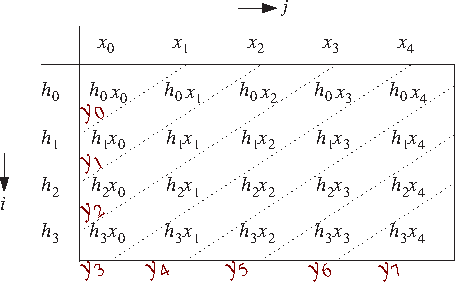
\includegraphics[width = 1\textwidth]{pic/convTab.pdf}
		\end{minipage}


	\subsection{LTI-Form Faltung }
		\begin{minipage}{0.37\textwidth}
		 	Der Eingangsvektor $x(n)$ kann in gewichtete und verzögerte Diracs aufgesplittet werden. Diese werden einzeln durch das LTI-System geschickt und deren gewichteten und verzögerten Impulsantworten summiert.
		 \end{minipage}\begin{minipage}{0.03\textwidth}$ $\end{minipage}
		 \begin{minipage}{0.62\textwidth}
		 	$\begin{array}{lcl}
		 	  x& = &x_0\,[\,1,\,0,\,0,\,0,\,0\,]\\
		 	   & + &x_1\,[\,0,\,1,\,0,\,0,\,0\,]\\
		 	   & + &x_2\,[\,0,\,0,\,1,\,0,\,0\,]\\
		 	   & + &x_3\,[\,0,\,0,\,0,\,1,\,0\,]\\
		 	   & + &x_4\,[\,0,\,0,\,0,\,0,\,1\,]\\
		 	 \end{array}\xrightarrow {\;\;\;H\;\;\;}
		 	 \begin{array}{lcl}
		 	  y& = &x_0\,[\,h_0,\,h_1,\,h_2,\,h_3,\,0,\,0,\,0,\,0\,]\\
		 	   & + &x_1\,[\,0,\,h_0,\,h_1,\,h_2,\,h_3,\,0,\,0,\,0\,]\\
		 	   & + &x_2\,[\,0,\,0,\,h_0,\,h_1,\,h_2,\,h_3,\,0,\,0\,]\\
		 	   & + &x_3\,[\,0,\,0,\,0,\,h_0,\,h_1,\,h_2,\,h_3,\,0\,]\\
		 	   & + &x_4\,[\,0,\,0,\,0,\,0,\,h_0,\,h_1,\,h_2,\,h_3\,]\\
		 	 \end{array}$
		\end{minipage}\\[0.2cm]

		\begin{minipage}{0.7\textwidth}
		 	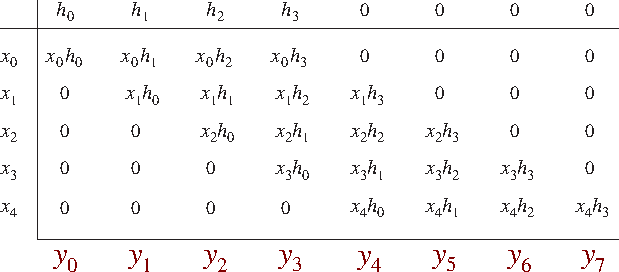
\includegraphics[width = 0.9\textwidth]{pic/LTITab.pdf}
		\end{minipage}
		\begin{minipage}{0.3\textwidth}
		 	\fcolorbox{CadetRed}{white}{$y(n) = \mysum{m}{}{x(m)\cdot h(n-m)}$}
		\end{minipage}
	\subsection{Matrix Form}
		Die Faltung zwischen Eingangsvektor $x(n)$ und Impulsantwort $h(n)$ kann auch als Matrixmultiplikation geschriben werden. Dabei gibt es zwei Formen:
		\begin{itemize}
		 \item Impulsantwortmatrix$\qquad\quad\;$\fcolorbox{CadetRed}{white}{$\vec y = H\cdot\vec x$}
		 \item Eingangssequenzmatirx $\qquad$\fcolorbox{CadetRed}{white}{$\vec y = X\cdot\vec h$}\\
		\end{itemize}
		
		\begin{minipage}{0.5\textwidth}
			\textbf{Impulsantwortmatrix \bm{$H\; ((L_x+M)\times L_x)$} }\\[0.2cm]
			$\begin{bmatrix} \;y_0\;\;\\y_1\\y_2\\y_3\\y_4\\y_5\\y_6\\y_7\end{bmatrix} = \underbrace{\begin{bmatrix} \;h_0\;\; & 0 & 0 & 0 & 0\\ h_1&\;h_0\;\;&0&0&0\\h_2&h_1&\;h_0\;\;&0&0\\h_3&h_2&h_1&\;h_0\;\;&0\\0&h_3&h_2&h_1&\;h_0\;\;\\0&0&h_3&h_2&h_1\\0&0&0&h_3&h_2\\0&0&0&0&h_3\end{bmatrix}}_{H}\cdot \begin{bmatrix} \;x_0\;\;\\x_1\\x_2\\x_3\\x_4\end{bmatrix}$
		\end{minipage}
		\begin{minipage}{0.5\textwidth}
			\textbf{Eingangssequenzmatirx \bm{$X\; ((L_x+M)\times (M+1))$} }\\[0.2cm]
			$\begin{bmatrix} \;y_0\;\;\\y_1\\y_2\\y_3\\y_4\\y_5\\y_6\\y_7\end{bmatrix} = \underbrace{\begin{bmatrix} \;x_0\;\; & 0 & 0 & 0\\ x_1&\;x_0\;\;&0&0\\x_2&x_1&\;x_0\;\;&0\\x_3&x_2&x_1&\;x_0\;\;\\x_4&x_3&x_2&x_1&\\0&x_4&x_3&x_2\\0&0&x_4&x_3&\\0&0&0&x_4&\end{bmatrix}}_{X}\cdot \begin{bmatrix} \;h_0\;\;\\h_1\\h_2\\h_3\end{bmatrix}$
		\end{minipage}
	
\newpage
	\subsection{Overlap-Add Blockfaltung}
		\vspace*{-0.2cm}\begin{minipage}{0.4\textwidth}
			Wenn die Eingangssequenz sehr lange wird muss diese in Blöcke der Länge $L_x$ aufgeteilt werden. Jeder dieser Blöcke wird einzeln verarbeitet. Da durch die Faltung aber Ausgangblöcke entstehen, die länger sind als die Eingangsblöcke, müssen diese auf die Länge der Eingangsblöcke $L_x$ zugeschnitten werden. der Rest des Ausgangsblockes $y_{temp}$ zum nächsten Blockes addiert.
		\end{minipage}
		\begin{minipage}{0.03\textwidth}$ $\end{minipage}
		\begin{minipage}{0.55\textwidth}
			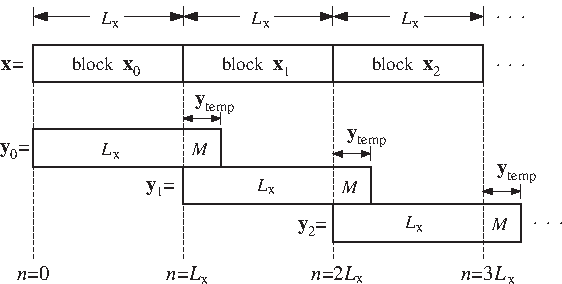
\includegraphics[width = 1\textwidth]{pic/overlapConv.pdf}
		\end{minipage}

	\subsection{Generelle Faltung}
		Für akausale Eingangssequenzen und akausale Impulsantworten gilt folgende allgemeine Faltungsformel:\\[0.2cm]
		\begin{minipage}{0.57\textwidth}
			Direct-Form:$\qquad$\fcolorbox{CadetRed}{white}{$y(n) = \mysum{m = max\{-M_1,n-L_2+1\}}{min\{n+L_1,M_2\}}{h(m)\cdot x(n-m)}$}\\[0.2cm]
		\end{minipage}
		\begin{minipage}{0.03\textwidth}$ $\end{minipage}
		\begin{minipage}{0.4\textwidth}
			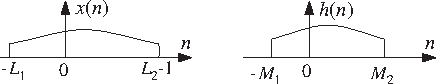
\includegraphics[width = 1\textwidth]{pic/genConv.pdf}
		\end{minipage}
		
	\subsection{DC-Gain}
		Der DC-Gain eines stabilen Filters ist der Wert, auf den der Ausgang konvergiert, wenn am Eingang der Einheitsschritt angelegt wird $x(n) = u(n)$\\[0.2cm]
		\textbf{DC-Gain}$\qquad$\fcolorbox{CadetRed}{white}{$y_{DC} = \mysum{m}{}{h(m)}$}\\[0.4cm]
		
\section{Sample für Sample Verarbeitung}
	\vspace*{-0.8cm}\begin{minipage}{0.65\textwidth}
		\begin{itemize}
		\item Die Sample für Sample Verarbeitung wird angewendet wenn zwischen Ein- und Ausgang nur eine kurze Verzögerungszeit liegen darf (Echtzeitsysteme).\\[-0.4cm]
		\item Diese Verarbeitung kann in Signalflussdiagrammen dargestellt werden. Dazu werden die drei Elemente Addierer, Verstärker und Verzögerer verwendet.
		\end{itemize}
	\end{minipage}
	\begin{minipage}{0.05\textwidth}$ $\end{minipage}
	\begin{minipage}{0.3\textwidth}
		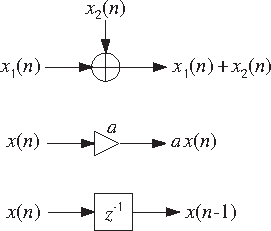
\includegraphics[width = 1\textwidth]{pic/sampleSample.pdf}
	\end{minipage}\\[-0.5cm]
		
	\subsection{Verzögerung (Pure Delays)}
		Um die verzögerte Werte speichern zu können werden \textbf{Zustände} definiert.\\ Ein Zustand $w(n)$ ist ein Register, welches den vorhergehenden Wert (Zustand) speichert. \\[0.2cm]
		\begin{danger}
		 Die Reihenfolge der Register-Updates ist sehr wichtig!
		\end{danger}\\[0.3cm]
		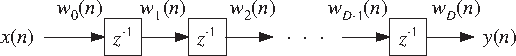
\includegraphics[width = 0.6\textwidth]{pic/delayD.pdf}\\[0.4cm]
		\begin{minipage}{0.3\textwidth}
			\textbf{I/O Gleichungen}\\[0.2cm]
			\begin{tabular}{|l|}
			\hline $ $\\[-0.3cm]
				$w_0(n) = x(n)$\\
				$y(n) = w_D(n)$\\[0.2cm]
				for $i = D,D-1,..,1$ do:\\
				$w_i(n+1) = w_{i-1}(n)$\\[0.2cm]
			\hline     
			\end{tabular}
		\end{minipage}
		\begin{minipage}{0.4\textwidth}
			\textbf{Algorithums}\\[0.2cm]
			\begin{tabular}{|l|}
			\hline $ $\\[-0.3cm]
				$w[0] = x;$\\
				$y = w[D]; $\\[0.2cm]
				for $i = D,D-1,..,1$ do:\\
				$w[i] = w[i-1];$\\[0.2cm]
			\hline     
			\end{tabular} 
		\end{minipage}

\newpage
	\subsection{FIR filtern mit Direktform}
		\begin{minipage}{0.5\textwidth}
			Die Direktform I/O Faltungsformel für ein FIR-Filter der Ordung $M$ lautet:\\[0.2cm]
			\fcolorbox{CadetRed}{white}{$\begin{array}{lcl}y(n)& =& h_0x(n) + h_1x(n-1) + ... + h_Mx(n-M)\\[0.2cm]& =& h_0w_0(n) + h_1w_1(n) + ... + h_Mw_M(n)\end{array}$}\\[0.4cm]
			Diese Form kann direkt in ein Signalflussdiagramm umgesetzt werden. Dabei gelten folgende Beziehungen:\\[0.2cm]
			\fcolorbox{CadetRed}{white}{$\begin{array}{l}w_0(n) = x(n)\\w_1(n) = x(n-1) = w_0(n-1)\\w_2(n) = x(n-2) = w_1(n-1)\\\vdots\\w_M(n) = x(n-M) = w_{M-1}(n-1)\end{array}$}
		\end{minipage}\begin{minipage}{0.03\textwidth}$ $\end{minipage}
		\begin{minipage}{0.4\textwidth}
			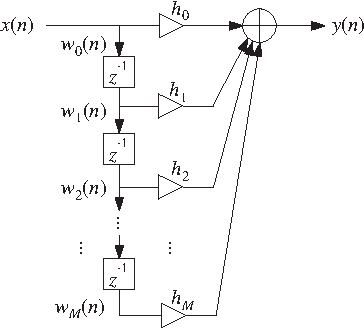
\includegraphics[width = \textwidth]{pic/firFlussdiagramm.pdf}
		\end{minipage}\\[0.2cm]

		\begin{itemize}
		 \item Durch die Verwendung von internen Zuständen kann der Ausgang aus dem aktuellen Eingangswert und den Zuständen berechnet werden.
		 \item Die input-on und input-off Transienten können anhand des Signalflussdiagrammes leicht erklärt werden. Sie entsprechen jeweils der Zeit (Anzahl Samples), bis die Verzögerungslinie (Zustände) gefüllt bzw. geleert sind.\\[-0.2cm]
		\end{itemize}
		\begin{minipage}{0.5\textwidth}
			\textbf{I/O Gleichungen}\\[0.2cm]
			\begin{tabular}{|l|}
			\hline $ $\\[-0.3cm]
				$w_0(n) = x(n)$\\
				$y(n) = h_0w_0(n) + h_1w_1(n) + ... + h_Mw_M(n)$\\[0.2cm]
				for $i = M,M-1,..,1$ do:\\
				$w_i(n+1) = w_{i-1}(n)$\\[0.2cm]
			\hline     
			\end{tabular}
		\end{minipage}
		\begin{minipage}{0.4\textwidth}
			\textbf{Algorithums}\\[0.2cm]
			\begin{tabular}{|l|}
			\hline $ $\\[-0.3cm]
				$w[0] = x;$\\
				$y = h[0]\,w[0] + h[1]\,w[1] + ... + h[M]\,w[M]; $\\[0.2cm]
				for $i = M,M-1,..,1$ do:\\
				$w[i] = w[i-1];$\\[0.2cm]
			\hline     
			\end{tabular} 
		\end{minipage}